\section{热功当量}\label{sec:5-5}

既然做功和热传递对改变物体的热能是等效的,那么功和热量之间是否有确定的数量关系呢?

最先研究这个关系的是英国物理学家焦耳。
他从十九世纪四十年代开始,花了大约四十年的时间,用各种不同的做功方法做了四百多次实验来研究这个关系。
以后又有许多人用更精确的方法来研究这个关系。
实验结果表明,功和热量之间存在着确定的数量关系:1 卡的热量跟 4.2 焦耳的功相当。
这个相当的关系在物理学上用
$$ 1\ka = 4.2 \jiaoer $$
来表示,它给出了热量的单位卡和功的单位焦耳之间的换算关系,叫做\textbf{热功当量}。

既然卡和焦耳这两个单位间存在确定的换算关系,就可以只保留一个,省去单位换算的麻烦;
现在的国际单位制正是这样。\CJKunderwave{国际单位制规定热量的单位跟功的单位一样,也是焦耳}。

焦耳不但是功和热量的单位,也是国际单位制中能量的单位。
各种形式的能,如机械能、热能、电能,单位都是焦耳。

热量的单位卡,是过去人们对功和热量相当的关系还不清楚的情况下规定的,现在已经可以废弃不用了。
不过因为卡这个单位长期沿用下来,要把以卡为单位的许许多多技术资料都改成以焦耳为单位,还需要一段时间。

\section*{阅读材料}

\begin{wrapfigure}[14]{r}{6cm}
    \centering
    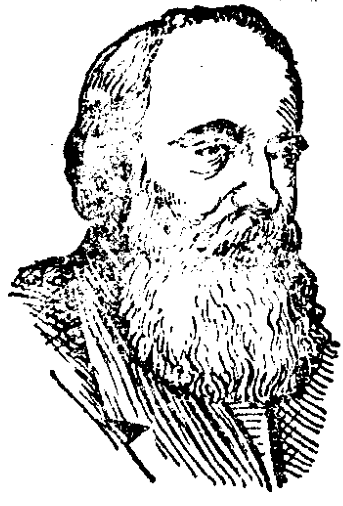
\includegraphics[width=5cm]{../pic/czwl2-ch5-joule}
    \caption*{焦耳(1818~1889)}\label{fig:5-joule}
\end{wrapfigure}

焦耳是英国物理学家。焦耳没有上过学,他的科学知识几乎全是靠自学获得的。
1840 年,他多次做了导体通过电流发热的实验。
根据实验结果,写出了他的第一篇科学论文《电流析热》,提出了电能转化为热能的规律。
这时焦耳才二十二岁。这个规律就是我们将在第九章学到的焦耳定律。

焦耳探讨了各种形式能的转化关系。1843 年 8 月,他在英国学术协会上作了《论电磁热效应和热功当量》的报告。
报告的结论是:自然界的能量是不能消灭的,消耗了机械能,总能得到相当的热能。

焦耳采用自己精心设计的量热器,测定了热量和功的数量关系,即热功当量。
焦耳的实验结果已经相当精确了,但是他不满足已有的成就,不断改进方法,继续进行实验,
从十九世纪四十年代开始到七十年代近四十年当中,用各种方法进行了四百多次实验。
他得到的热功当量的数值,保持了三十年没有较大的变化,这在物理学史上是极为罕见的。


